\documentclass[a4 paper, 12pt]{report}
\usepackage[utf8]{inputenc}
\usepackage{indentfirst}
	\setlength{\parindent}{2.30em}
\setcounter{tocdepth}{3}
\setcounter{secnumdepth}{3}
\usepackage{pdflscape}
\usepackage{subfigure}
\usepackage{rotating}
\usepackage{wrapfig}
\usepackage{lscape}
\usepackage{booktabs,tabularx}
\usepackage{lscape}
\usepackage{mathptmx}
\usepackage{amsmath,amssymb,amsfonts}
\usepackage{wasysym}
\usepackage{bm}
\usepackage{xfrac}
\usepackage{lipsum}
\usepackage[top=4.572cm, bottom=3.175cm, left=3.81cm, right=3.175cm]{geometry}
\usepackage{sectsty}  % section font size
	\sectionfont{\normalsize}
	\subsectionfont{\normalsize}
	\subsubsectionfont{\normalsize}
	\paragraphfont{\normalsize}
	\subparagraphfont{\normalsize}
\usepackage{etoolbox} % remove spaces before and after paragraph
\usepackage{setspace} % control linespacing
	\setstretch{1.5}
\usepackage{natbib}
\bibliographystyle{apalike}
\usepackage{graphicx}
	\graphicspath{{./Figure/}}
	\DeclareGraphicsExtensions{.pdf,.jpeg,.jpg,.png}
\usepackage{textcomp}
\usepackage[dvipsnames]{xcolor}
\usepackage{caption}
\captionsetup{format=hang, font=normalsize, labelfont=bf, justification=justified, labelsep=period}
% Pagination
\usepackage{fancyhdr}
	\pagestyle{fancyplain}% <- use fancyplain instead fancy
	\fancyhf{}
	\fancyhead[R]{\thepage}
	\renewcommand{\headrulewidth}{0pt}
% Algorithm
\usepackage[ruled,vlined,linesnumbered,resetcount,algochapter]{algorithm2e}
% Table
\usepackage{multirow}
% Icons
\usepackage{fontawesome}
% Hyperlinks
\usepackage{hyperref} 
\usepackage{cleveref}
\makeatletter
	\patchcmd{\@makechapterhead}{\vspace*{60\p@}}{}{}{}% Removes space above \chapter head
	\patchcmd{\@makeschapterhead}{\vspace*{50\p@}}{}{}{}% Removes space above \chapter* head
	\chapterfont{\normalsize \centering \MakeUppercase}
\numberwithin{equation}{chapter}
\makeatother
% Table of Contents and References
\usepackage[english]{babel}
\addto\captionsenglish{% Replace "english" with the language you use
  \renewcommand{\contentsname}%
    {Table of Contents}%
  \renewcommand{\bibname}{References}
}
\thispagestyle{empty} 
\begin{document}


    %  Comment line if you want to hide from the presentation

    %%%%%%%%%%%%%%%%%%%%%%%%%%%%%%%%%%%%%%%%%%%%%%%%%%%%%%%%%%%%%%%%%%%%%%%%%%
% TITLE PAGE 
%%%%%%%%%%%%%%%%%%%%%%%%%%%%%%%%%%%%%%%%%%%%%%%%%%%%%%%%%%%%%%%%%%%%%%%%%%

       \phantomsection
       \addcontentsline{toc}{chapter}{TITLE PAGE}

       \begin{center}
       \textbf{A LATEX TEMPLATE OF A MANUSCRIPT FOR THE BACHELOR OF SCIENCE IN COMPUTER ENGINEERING PROGRAM}

       \vspace{2cm}
            AN UNDERGRADUATE THESIS
       
       \vspace{2cm}  
            Presented to the\\  
            Department of Computer Engineering and Mechatronics\\ 
            College of Engineering\\
            MSU-Iligan Institute of Technology\\ 
            Iligan City

      \vspace{2cm}      
          In Partial Fulfillment\\ 
          of the Requirements for the Degree\\ 
          BACHELOR OF SCIENCE IN COMPUTER ENGINEERING

     \vspace{2cm}

        \textbf{EARL RYAN M. ALELUYA}\\
        \vspace{2cm}

        September 2025
            
   \end{center}
    %%%%%%%%%%%%%%%%%%%%%%%%%%%%%%%%%%%%%%%%%%%%%%%%%%%%%%%%%%%%%%%%%%%%%%%
% CERTIFICATION OF PANEL APPROVAL
%%%%%%%%%%%%%%%%%%%%%%%%%%%%%%%%%%%%%%%%%%%%%%%%%%%%%%%%%%%%%%%%%%%%%%%

\pagenumbering{roman} 

\setstretch{1}

\chapter*{}
    \thispagestyle{empty}


    \begin{table}[ht]
        \begin{tabular}{ll}
        \multirow{5}{*}{
\includegraphics[width=1in]{images/msuiit_logo.png}} 
                             & \quad \textbf{Mindanao State University} \\
                             & \quad \textbf{ILIGAN INSTITUTE OF TECHNOLOGY}    \\
                             & \quad \textit{College of Engineering}   \\
                             & \quad Andres Bonifacio Avenue, Tibanga, \\
                             & \quad Iligan City 9200, Philippines  
        \end{tabular}
    \end{table}

    \begin{center}
        \textbf{CERTIFICATION OF PANEL APPROVAL}   
    \end{center}


    
    The undergraduate thesis attached hereto, titled 
    \textbf{
        "A LATEX TEMPLATE OF A MANUSCRIPT FOR THE BACHELOR OF SCIENCE IN COMPUTER ENGINEERING PROGRAM"
    } 
    prepared and submitted by 
    \textbf{
        EARL RYAN M. ALELUYA
    },
    in partial fulfillment for the degree of \textbf{BACHELOR OF SCIENCE IN COMPUTER ENGINEERING}, is hereby recommended for approval:


    
    \begin{table}[ht]
        \centering
        \begin{tabular}{cc}
        
        \begin{tabular}[c]{@{}c@{}}\\
            \textbf{\underline{PROF. CHERRY MAE G. VILLAME}}
            \\ Member\\ \rule{3cm}{1pt}\\ Date\end{tabular} &
       
        \begin{tabular}[c]{@{}c@{}}\\
        \textbf{\underline{PROF. STEPHEN H. HAIM}}
        \\ Member\\ \rule{3cm}{1pt}\\ Date\end{tabular} \\
        
        \multicolumn{2}{c}{\begin{tabular}[c]{@{}c@{}} \\ \\
            \textbf{\underline{PROF. FRANCIS JANN A. ALAGON}}
            \\ Adviser\\ \rule{3cm}{1pt}\\ Date\end{tabular}}


        %   \begin{tabular}[c]{@{}c@{}}\\
        %     \textbf{\underline{PROF. CHERRY MAE G. VILLAME}}
        %     \\ Member\\ \rule{3cm}{1pt}\\ Date\end{tabular} &
       
        % \begin{tabular}[c]{@{}c@{}}\\
        %     \textbf{\underline{PROF. STEPHEN H. HAIM}}
        %     \\ Adviser\\ \rule{3cm}{1pt}\\ Date\end{tabular} \\
        
        \end{tabular}
    \end{table}
    
   This undergraduate thesis is approved in partial fulfillment of the requirements for the degree of \textbf{BACHELOR OF SCIENCE IN COMPUTER ENGINEERING}.

    \begin{table}[ht]
        \centering
        \begin{tabular}{c}
        \begin{tabular}[c]{@{}c@{}} \\
        
        \textbf{\underline{PROF. FRANCIS JANN A. ALAGON}}
        \\ Chair, Department of Computer Engineering and Mechatronics\\ \rule{3cm}{1pt}\\ Date\end{tabular} \\
        \begin{tabular}[c]{@{}c@{}} \\ \\
        
        \textbf{\underline{PROF. JEFFERSON A. HORA, Ph.D.}}
        \\ Dean, College of Engineering\\ \rule{3cm}{1pt}\\ Date\end{tabular}
        \end{tabular}
    \end{table}
   
    
\phantomsection
\addcontentsline{toc}{chapter}{CERTIFICATION OF PANEL APPROVAL}
    %%%%%%%%%%%%%%%%%%%%%%%%%%%%%%%%%%%%%%%%%%%%%%%%%%%%%%%%%%%%%%%%%%%%%%%
% ABSTRACT
%%%%%%%%%%%%%%%%%%%%%%%%%%%%%%%%%%%%%%%%%%%%%%%%%%%%%%%%%%%%%%%%%%%%%%%
\setstretch{1.5}
\chapter*{ABSTRACT}
    A single paragraph of about 200 words maximum. An abstract should give a pertinent overview of the work. We strongly encourage authors to use the following style of structured abstracts, but without headings: (1) Background: Place the question addressed in a broad context and highlight the purpose of the study; (2) Methods: briefly describe the main methods or treatments applied; (3) Results: summarize the article’s main findings; (4) Conclusions: indicate the main conclusions or interpretations. The abstract should be an objective representation of the article, must not contain results not presented and substantiated in the main text, and should not exaggerate the main conclusions.

    \noindent
    \textbf{Keywords | } Keyword 1; Keyword 2; 
    \textit{(List 3 to 6 pertinent keywords related to the subject discipline. You can refer to \href{https://www.ieee.org/content/dam/ieee-org/ieee/web/org/pubs/ieee-taxonomy.pdf}{\textcolor{blue}{IEEE Taxonomy}}) }

\phantomsection
\addcontentsline{toc}{chapter}{ABSTRACT}
    %%%%%%%%%%%%%%%%%%%%%%%%%%%%%%%%%%%%%%%%%%%%%%%%%%%%%%%%%%%%%%%%%%%%%%%
% ACKNOWLEDGMENT
%%%%%%%%%%%%%%%%%%%%%%%%%%%%%%%%%%%%%%%%%%%%%%%%%%%%%%%%%%%%%%%%%%%%%%%
\chapter*{ACKNOWLEDGMENT}
    The BS Computer Engineering Faculty Members made this template. Special acknowledgment to the leading contributors: Asst. Prof. Earl Ryan Aleluya, Asst. Prof. Francis Jann Alagon, and Engr. Stephen Haim. 

\phantomsection
\addcontentsline{toc}{chapter}{ACKNOWLEDGMENT}
    %%%%%%%%%%%%%%%%%%%%%%%%%%%%%%%%%%%%%%%%%%%%%%%%%%%%%%%%%%%%%%%%%%%%%%%
% TABLE OF CONTENTS
%%%%%%%%%%%%%%%%%%%%%%%%%%%%%%%%%%%%%%%%%%%%%%%%%%%%%%%%%%%%%%%%%%%%%%%


\tableofcontents
%\phantomsection
%\addcontentsline{toc}{chapter}{TABLE OF CONTENTS}

\listoffigures
\phantomsection
\addcontentsline{toc}{chapter}{LIST OF FIGURES}

\listoftables
\phantomsection
\addcontentsline{toc}{chapter}{LIST OF TABLES}

\listofalgorithms
\phantomsection
\addcontentsline{toc}{chapter}{LIST OF ALGORITHMS}
    %%%%%%%%%%%%%%%%%%%%%%%%%%%%%%%%%%%%%%%%%%%%%%%%%%%%%%%%%%%%%%%%%%%%%%%
%---------------------------------------------------------------------%
% Start of CHAPTER 1 INTRODUCTION
%---------------------------------------------------------------------%
%%%%%%%%%%%%%%%%%%%%%%%%%%%%%%%%%%%%%%%%%%%%%%%%%%%%%%%%%%%%%%%%%%%%%%%
\renewcommand{\thechapter}{\Roman{chapter}}
\chapter{Introduction}
    \thispagestyle{empty} 
    \pagenumbering{arabic} 
    \label{ch:Introduction}
    \renewcommand{\thechapter}{\arabic{chapter}}


%%%%%%%%%%%%%%%%%%%%%%%%%%%%%%%%%%%%%%%%%%%%%%%%%%%%%%%%%%%%%%%%%%%%%%%
% SECTION 1.1 BACKGROUND OF THE STUDY
%%%%%%%%%%%%%%%%%%%%%%%%%%%%%%%%%%%%%%%%%%%%%%%%%%%%%%%%%%%%%%%%%%%%%%%

\section{Background of the Study}
    \label{sec:Background of the Study}

    This document is a model and instructions for \LaTeX.  Please observe the proper format.

    First, this is how you cite a reference \citep{aleluya2018decision}. Notice that the bibliography in the last portion of this template will be created automatically, following an APA citation style. Use BibTex for storing all your references.

    Second, this is how you cite a section/subsection in your paper. For example: The reader must refer to Section \ref{sec:Background of the Study}.

    Third, this is how you cite an appendix. For example: The reader must refer to Appendix \ref{ap:Appendix A}.

    Fourth, this is how you write an equation.
        \begin{equation}
            \label{eq:pythagoras}
            c^2 = a^2+b^2
        \end{equation}
    
    This is an example of how to cite the equation in the paper following APA style. Equation \ref{eq:pythagoras} presents the formula for Pythagoras Theorem.
    

    Fifth, this is how you write a table following APA style. You can use online LaTex table generator to make your life easier.
        \begin{table}[ht]
            \caption{Descriptive Statistics for Sample Data}
            \label{tab:descriptive_stats}
            \centering
            \begin{tabular}{lccc}
                \hline
                & \textbf{Mean} & \textbf{SD} & \textbf{N} \\
                \hline
                Variable 1 & 25.6 & 3.2 & 100 \\
                Variable 2 & 18.7 & 2.8 & 100 \\
                Variable 3 & 30.2 & 4.5 & 100 \\
                \hline
            \end{tabular}
        \end{table}

    This is an example of how to cite the table in the paper. Table \ref{tab:descriptive_stats} presents the descriptive statistics for several sample data from the population. Notice that the \textit{List of Tables} will be generated automatically.


    Sixth, this is how you write an Algorithm in the paper following an APA style. 
        \begin{algorithm}[ht]
            \caption{Example Algorithm}
            \label{alg:example}
            
            \KwData{Input data}
            \KwResult{Output result}
            \While{condition}{
                Perform action\;
                \If{conditional}{
                    Do something\;
                }
                \Else{
                    Do another thing\;
                }
            }            
            \For{each element in collection}{
                Process element\;
            }    
        \end{algorithm}

    This is an example of how to cite the algorithm in the paper. Algorithm \ref{alg:example} presents a sample algorithm. Notice that the \textit{List of Algorithms} will be generated automatically.


    Lastly, this is how you import figures in the paper, with the caption that follows APA style.
        \begin{figure}[ht]
        	\centering
        	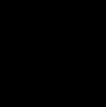
\includegraphics[scale = 0.70]{images/blackbox.png}
            \caption{
        			Black box
        	}
            \label{fig:blackbox}
        \end{figure}

    This is an example of how to cite the figure in the paper. Figure \ref{fig:blackbox} illustrates a sample imported image of a black box. Notice that the \textit{List of Figures} will be generated automatically.


    So far, what do you think? Now, you can start writing your manuscript. I would like you to please read the description in each section to gain an idea of what to write. Please feel free to research online if you need more information.

    \textbf{What is background of the study?}
    The background of the study is a section in a thesis where you provide context and justification for your research. This section typically answers the "why" of your research by explaining the problem or gap in knowledge that your research addresses.

%%%%%%%%%%%%%%%%%%%%%%%%%%%%%%%%%%%%%%%%%%%%%%%%%%%%%%%%%%%%%%%%%%%%%%%
% SECTION 1.2 STATEMENT OF THE PROBLEM
%%%%%%%%%%%%%%%%%%%%%%%%%%%%%%%%%%%%%%%%%%%%%%%%%%%%%%%%%%%%%%%%%%%%%%%
    
\section{Statement of the Problem}
    \label{sec:Statement of the Problem}

    A problem statement is an explanation in research that describes the issue that needs study. What problem is the research attempting to address? It is expected to be brief and concise and should not include the findings of the research or detailed data. It shall define the problem, which can be thought of as a gap in the information base. There may be several solutions to this gap or a need for more information, but that is not the concern of the problem statement. Its purpose is to summarize the current information and where a lack of knowledge may present a problem that must be investigated. The purpose of the problem statement is to identify the issue that is a concern and focus it in a way that allows it to be studied systematically. It defines the problem and demonstrates why further information is needed for a solution to become possible.


%%%%%%%%%%%%%%%%%%%%%%%%%%%%%%%%%%%%%%%%%%%%%%%%%%%%%%%%%%%%%%%%%%%%%%%
% SECTION 1.3 OBJECTIVES OF THE STUDY
%%%%%%%%%%%%%%%%%%%%%%%%%%%%%%%%%%%%%%%%%%%%%%%%%%%%%%%%%%%%%%%%%%%%%%%

\section{Objectives of the Study}
    \label{sec:Objectives of the Study}

    \par The general objective is to . The specific objectives are as follows:
    
    \begin{enumerate}
    	\item To ;
    	\item To ; and
    	\item To .
    \end{enumerate}

%%%%%%%%%%%%%%%%%%%%%%%%%%%%%%%%%%%%%%%%%%%%%%%%%%%%%%%%%%%%%%%%%%%%%%%
% SECTION 1.4 ORIGINALITY OF THE STUDY
%%%%%%%%%%%%%%%%%%%%%%%%%%%%%%%%%%%%%%%%%%%%%%%%%%%%%%%%%%%%%%%%%%%%%%%

\section{Originality of the Study}
\label{sec:Originality of the Study}

    The author should highlight and articulate the unique contributions and novel aspects of the research. This section must differentiate it from the existing literature.


%%%%%%%%%%%%%%%%%%%%%%%%%%%%%%%%%%%%%%%%%%%%%%%%%%%%%%%%%%%%%%%%%%%%%%%
% SECTION 1.5 SCOPES AND LIMITATIONS
%%%%%%%%%%%%%%%%%%%%%%%%%%%%%%%%%%%%%%%%%%%%%%%%%%%%%%%%%%%%%%%%%%%%%%%

\section{Scope and Limitations}
    \label{sec:Scope and Limitations}

    The author needs to outline the boundaries and constraints of the study. This section helps readers understand the extent of the research and the potential limitations that may affect the interpretation of the findings.


%%%%%%%%%%%%%%%%%%%%%%%%%%%%%%%%%%%%%%%%%%%%%%%%%%%%%%%%%%%%%%%%%%%%%%%
% SECTION 1.6 SIGNIFICANCE OF THE STUDY
%%%%%%%%%%%%%%%%%%%%%%%%%%%%%%%%%%%%%%%%%%%%%%%%%%%%%%%%%%%%%%%%%%%%%%%
    
\section{Significance of the Study}
    \label{sec:Significance of the Study}

    For the problem statement being tackled, the results of this study will benefit the following sectors:
    
    \begin{itemize}
        \item\textbf{Benefactor 1}.
         Explain why the study benefits Benefactor 1.
         
    	\item\textbf{Benefactor 2}.
         Explain why the study benefits Benefactor 2.
     
    	\item\textbf{Benefactor 3}.
         Explain why the study benefits Benefactor 3.
    \end{itemize}


%%%%%%%%%%%%%%%%%%%%%%%%%%%%%%%%%%%%%%%%%%%%%%%%%%%%%%%%%%%%%%%%%%%%%%%
% SECTION 1.7 CONCEPTUAL FRAMEWORK
%%%%%%%%%%%%%%%%%%%%%%%%%%%%%%%%%%%%%%%%%%%%%%%%%%%%%%%%%%%%%%%%%%%%%%%

\section{Conceptual Framework}
    \label{sec:Conceptual Framework}
    
    The conceptual framework is a critical research study component that outlines the theoretical foundation and key concepts guiding the investigation. It serves as a roadmap for understanding the relationships between variables and helps researchers formulate hypotheses and design the study. In this section, it is essential to explain the theoretical perspectives, existing models, and relevant literature that inform the study's approach. Additionally, the conceptual framework should elucidate the researcher's assumptions, define key terms, and highlight the conceptual boundaries of the study. By establishing a clear and comprehensive conceptual framework, researchers provide a solid foundation for their work, enabling readers to contextualize the study within the broader academic landscape and grasp the theoretical underpinnings guiding their research endeavors.

    If the study is part of a bigger project, you need to illustrate what portion of the project you are focusing on. You can present the general concept of the project to provide the reader with the big picture. Also, you can present a detailed idea of your study so that it is easy to understand your scope. Please make up your thoughts and divide them by discussing them in different subsections.

    \subsection{Insert Title}
        Lorem Ipsum.
    
    \subsection{Insert Title}
        Lorem Ipsum.


%%%%%%%%%%%%%%%%%%%%%%%%%%%%%%%%%%%%%%%%%%%%%%%%%%%%%%%%%%%%%%%%%%%%%%%
% SECTION 1.8 DEFINITION OF TERMS
%%%%%%%%%%%%%%%%%%%%%%%%%%%%%%%%%%%%%%%%%%%%%%%%%%%%%%%%%%%%%%%%%%%%%%%

\section{Definition of Terms}
    \label{sec:Definition of Terms}

    The following terms are used throughout the study:

    \begin{enumerate}
        \item 
            \textbf{LaTeX} \textemdash is a software system for typesetting documents. It describes the content and layout of the document.
        \item 
            \textbf{Note} \textemdash please arrange your terms alphabetically.
    \end{enumerate}

    %%%%%%%%%%%%%%%%%%%%%%%%%%%%%%%%%%%%%%%%%%%%%%%%%%%%%%%%%%%%%%%%%%%%%%%
%---------------------------------------------------------------------%
% Start of CHAPTER 2 REVIEW OF RELATED LITERATURE
%---------------------------------------------------------------------%
%%%%%%%%%%%%%%%%%%%%%%%%%%%%%%%%%%%%%%%%%%%%%%%%%%%%%%%%%%%%%%%%%%%%%%%
     
\renewcommand{\thechapter}{\Roman{chapter}}
\chapter{Review of Related Literature}
    \thispagestyle{empty} 
    \renewcommand{\thechapter}{\arabic{chapter}}

    The review of related literature synthesizes and evaluates existing scholarly works relevant to the study's topic. It involves a comprehensive examination of peer-reviewed articles, books, and other academic sources, with the aim of identifying gaps, trends, and insights related to the research questions. This section not only provides a historical context for the study but also helps establish the significance of the research by demonstrating the current state of knowledge in the field. Researchers highlight key findings, methodologies, and theoretical frameworks from previous studies to contextualize their own work and justify its contribution to the existing body of knowledge. A well-structured review of related literature not only informs the reader about the existing research landscape but also lays the groundwork for developing a robust conceptual framework and research methodology.

    \textit{Important Note:} Please outline your RRL based on your objectives. Ask for guidance from your COE194 instructor, adviser, or panel member.

\section{Review for Objective/Phase 1}
    The.

\section{Review for Objective/Phase 2}
    The.

\section{Review for Objective/Phase 3}
    The.

\section{Summary}
    The summary should briefly synthesize the related studies. It aims to highlight the gaps and the novelty of the proposed solution.
    %%%%%%%%%%%%%%%%%%%%%%%%%%%%%%%%%%%%%%%%%%%%%%%%%%%%%%%%%%%%%%%%%%%%%%%
%---------------------------------------------------------------------%
% Start of CHAPTER 3 METHODOLOGY
%---------------------------------------------------------------------%
%%%%%%%%%%%%%%%%%%%%%%%%%%%%%%%%%%%%%%%%%%%%%%%%%%%%%%%%%%%%%%%%%%%%%%%

\renewcommand{\thechapter}{\Roman{chapter}}
\chapter{Methodology}
    \thispagestyle{empty} 
    \renewcommand{\thechapter}{\arabic{chapter}}

    The research methodology section outlines the systematic approach and procedures to investigate the research questions or hypotheses. It encompasses the study's overall design, including the research paradigm, sampling techniques, data collection methods, and data analysis procedures. A detailed explanation of the chosen methodology, whether qualitative, quantitative, or mixed-methods approach, is provided, justifying its appropriateness for addressing the research objectives. The section also discusses ethical considerations, reliability, and validity measures, enhancing the transparency and credibility of the research. By elucidating the step-by-step process undertaken to gather and analyze data, the research methodology provides a blueprint for replication, allowing others in the field to assess the study's rigor and draw meaningful comparisons with similar research endeavors.

    \textit{Important Note:} Please outline your Methodology based on your objectives. Ask for guidance from your COE194 instructor, adviser, or panel member.

\section{Research Design}
    Lorem Ipsum.

\section{Research Methodology}
    Lorem Ipsum.

\subsection{Methods and Materials for Objective/Phase 1}
    Lorem Ipsum.

\subsection{Methods and Materials for Objective/Phase 2}
    Lorem Ipsum.

\subsection{Methods and Materials for Objective/Phase 3}
    Lorem Ipsum.


    %%%%%%%%%%%%%%%%%%%%%%%%%%%%%%%%%%%%%%%%%%%%%%%%%%%%%%%%%%%%%%%%%%%%%%%
%---------------------------------------------------------------------%
% Start of CHAPTER 4 RESULTS AND DISCUSSION
%---------------------------------------------------------------------%
%%%%%%%%%%%%%%%%%%%%%%%%%%%%%%%%%%%%%%%%%%%%%%%%%%%%%%%%%%%%%%%%%%%%%%%

\renewcommand{\thechapter}{\Roman{chapter}}
\chapter{Results and Discussion}
    \thispagestyle{empty} 
    \renewcommand{\thechapter}{\arabic{chapter}}

    In this section, you will need to present and interpret your research findings. Begin by objectively reporting the results, using clear and concise language, tables, or figures to support your observations. Discuss the significance of the research question or hypothesis results, addressing any unexpected findings and their potential implications. Compare your results with relevant literature, highlighting similarities or differences. Consider the limitations of your study and suggest areas for future research. Engage in thoughtful analysis, providing context for the results and offering insights contributing to the topic's broader understanding. Encourage the reader to critically evaluate the study and its contributions while maintaining a logical flow between the presentation of results and their discussion. 

\section{Results and Discussion for Objective/Phase 1}
    Lorem Ipsum.

\section{Results and Discussion for Objective/Phase 2}
    Lorem Ipsum.

\section{Results and Discussion for Objective/Phase 3}
    Lorem Ipsum.

    %%%%%%%%%%%%%%%%%%%%%%%%%%%%%%%%%%%%%%%%%%%%%%%%%%%%%%%%%%%%%%%%%%%%%%%
%---------------------------------------------------------------------%
% Start of CHAPTER 5 CONCLUSION AND RECOMMENDATIONS
%---------------------------------------------------------------------%
%%%%%%%%%%%%%%%%%%%%%%%%%%%%%%%%%%%%%%%%%%%%%%%%%%%%%%%%%%%%%%%%%%%%%%%

\renewcommand{\thechapter}{\Roman{chapter}}
\chapter{Conclusion and Recommendations}
    \thispagestyle{empty} 
    \renewcommand{\thechapter}{\arabic{chapter}}

    This chapter presents the conclusion the researcher has come up with and some recommendations beneficial to future researchers interested in continuing or improving this study.


\section{Conclusion}
    In the "Conclusion" section, summarize the key findings of your study, emphasizing their significance in the context of the research question or objectives. Avoid introducing new information but rather focus on the primary outcomes. Discuss how your results contribute to existing knowledge in the field and address the initial research objectives. Conclude with a concise statement that reinforces the overall importance of your work.

    \textit{Important Note:} Make sure that you conclude each objective of your study.

    Optionally, include any unexpected findings and their potential impact.

\section{Recommendations}
    In the "Recommendations" section, provide practical suggestions based on your study's findings. Offer guidance for future research or propose actionable steps that can be taken based on your results. Discuss potential applications or implications of your findings in relevant contexts. Address any limitations of your study and suggest ways in which future research can build upon or address these limitations. Your recommendations should be grounded in the evidence presented in your research and provide value to researchers and practitioners in the field.

    %%%%%%%%%%%%%%%%%%%%%%%%%%%%%%%%%%%%%%%%%%%%%%%%%%%%%%%%%%%%%%%%%%%%%%%
%---------------------------------------------------------------------%
% Start of BIBLIOGRAPHY
% (Automatically generated if you use \citep{} )
%---------------------------------------------------------------------%
%%%%%%%%%%%%%%%%%%%%%%%%%%%%%%%%%%%%%%%%%%%%%%%%%%%%%%%%%%%%%%%%%%%%%%%


\bibliography{References}
\phantomsection
\addcontentsline{toc}{chapter}{REFERENCES}
    %%%%%%%%%%%%%%%%%%%%%%%%%%%%%%%%%%%%%%%%%%%%%%%%%%%%%%%%%%%%%%%%%%%%%%%
%---------------------------------------------------------------------%
% Start of APPENDIX
%---------------------------------------------------------------------%
%%%%%%%%%%%%%%%%%%%%%%%%%%%%%%%%%%%%%%%%%%%%%%%%%%%%%%%%%%%%%%%%%%%%%%%

\appendix

\chapter{First Attachment Title}

    \label{ap:Appendix A}
    This is the content of Appendix A.

    \section{Additional Details}
        Some additional details go here.

\chapter{Second Attachment Title}
    \label{ap:Appendix B}
    This is the content of Appendix B.
    %%%%%%%%%%%%%%%%%%%%%%%%%%%%%%%%%%%%%%%%%%%%%%%%%%%%%%%%%%%%%%%%%%%%%%%
%---------------------------------------------------------------------%
% CURRICULUM VITAE
%---------------------------------------------------------------------%
%%%%%%%%%%%%%%%%%%%%%%%%%%%%%%%%%%%%%%%%%%%%%%%%%%%%%%%%%%%%%%%%%%%%%%%

\newpage
\thispagestyle{empty}

\phantomsection
\addcontentsline{toc}{chapter}{CURRICULUM VITAE}

\begin{table}[ht]
    \label{tab:cv-personal-info}
    \begin{tabular}{ll}
    \multirow{3}{*}{
\includegraphics[width=1.2in]{images/gradpic_no-cap.jpg}} 
                         & \textbf{\large EARL RYAN M. ALELUYA} \\
                         & \faMapO{} Iligan City 9200, Philippines              \\
                         & \faEnvelopeO{} earlryan.aleluya@g.msuiit.edu.ph               
    \end{tabular}
\end{table}

\setstretch{1.2}

%%%%%%%%%%%%%%%%%% EDUCATION %%%%%%%%%%%%%%%%%% 

\vspace{3em}
\section*{\faGraduationCap{} EDUCATION}
    \noindent
    \textbf{\small Bachelor of Science in Computer Engineering} \hfill \textit{June 20XX - May 20XX} \\
    \small MSU-Iligan Institute of Technology, Iligan City 9200, PH \\
    \small \textit{Cum Laude} 
    
    \vspace{1em} \noindent
    \textbf{\small Abcde National High School} \hfill \textit{June 20XX - May 20XX} \\
    \small Address

    \vspace{1em} \noindent
    \textbf{\small Abcde Elementary School} \hfill \textit{June 20XX - May 20XX} \\
    \small Address


%%%%%%%%%%%%%%%%%% EXPERIENCE %%%%%%%%%%%%%%%%%%

\section*{\faKey{} EXPERIENCE}
    \noindent
    \textbf{Job Title} \hfill \textit{Month Year - Present} \\
    Company Name, City, State \\

    \noindent
    \textbf{Internship Title} \hfill \textit{Month Year - Month Year} \\
    Internship Company, City, State \\


%%%%%%%%%%%%%%%%%% AWARDS AND ACHIEVEMENTS %%%%%%%%%%%%%%%%%%

\section*{\faTrophy{} AWARDS AND ACHIEVEMENTS}
    \noindent
    \textbf{Award Title} \hfill \textit{Month Year} \\
    Description of the award.

%%%%%%%%%%%%%%%%%% SKILLS %%%%%%%%%%%%%%%%%%

\section*{\faCode{} SKILLS}
    \noindent
    Skill 1  \quad Skill 2 \newline  
    Skill 3  \quad Skill 4


    
\end{document}